% !TEX encoding = IsoLatin2
\documentclass{pracamgren}

\usepackage[cmex10]{amsmath} \interdisplaylinepenalty=2500
\usepackage{amssymb,amsfonts,textcomp} \usepackage{amsthm}
\usepackage{latexsym}
%\usepackage[pdftex,pdfborder={0 0 0}]{hyperref}
\usepackage[utf8]{inputenc} \usepackage[T1]{fontenc}
%\usepackage[plmath,OT4]{polski}
\usepackage[pdftex]{color, graphicx} \usepackage{subfigure} \usepackage{svn}
\usepackage[naturalnames]{hyperref} \usepackage[lined, ruled, commentsnumbered,
linesnumbered]{algorithm2e}
\usepackage{multirow}

%\sloppy

%\usepackage[plain]{algorithm}

\hyphenation{Da-ta-Ca-ta-log}

%\usepackage[noend]{algpseudocode}


% remove after compressing the paper \raggedbottom

%\addtolength{\textfloatsep}{-5mm}

%\usepackage[noend,ruled]{algorithm2e}

% \usepackage{cite}
\usepackage[numbers]{natbib}

\newcommand{\fixme}[1]{{ {\em{\bf[FIXME: #1]}}}} 
\newcommand{\com}[1]{ {\em[Comment: #1]}} 
\newcommand{\todo}[1]{ {\bf \em [Todo: #1]}}
\newcommand{\smieci}[1]{}
\newcommand{\citept}[1]{}
%\newcommand{\fixme}[1]{}
\DeclareMathOperator*{\argmin}{arg\,min} \DeclareMathOperator*{\Var}{Var}

\mathchardef\mhyphen="2D

\author{Bolesław Kulbabiński}

\nralbumu{277531}

\title{Data replication in peer-to-peer storage systems}

\tytul{Replikacja danych w systemach peer-to-peer.}

\kierunek{Informatics}

\opiekun{Krzysztof Rządca Ph.D.}

\date{November 2014}

%Poda�? dziedzin�? wg klasyfikacji Socrates-Erasmus:
\dziedzina{ 
%11.0 Matematyka, Informatyka:\\ 11.1 Matematyka\\ 11.2 Statystyka\\ 
11.3 Informatyka\\ 
%11.4 Sztuczna inteligencja\\ 11.5 Nauki aktuarialne\\ 11.9 Inne nauki
%matematyczne i informatyczne
}

\dziedzinaang{
%11.0 Mathematics, Informatics:\\ 11.1 Mathematics\\ 11.2 Statistics\\ 11.3
Informatics, Computer Science\\ 
%11.4 Artificial Intelligence\\ 
%11.5 Actuarial Science\\ 11.9 Others Mathematics, Informatics
}

%Klasyfikacja tematyczna wedlug AMS (matematyka) lub ACM (informatyka)
\klasyfikacja{C. Organizacja systemów komputerów\\ C.2 Komputerowe sieci
komunikacyjne\\ C.2.4 Systemy rozproszone}


\klasyfikacjaang{C. Computer Systems Organization\\C.2 COMPUTER-COMMUNICATION NETWORKS \\
C.2.4 Distributed systems}

% S??owa kluczowe:
\keywords{systemy rozproszone, DHT, backup, zarządzanie zasobami}

\keywordsang{distributed systems, DHT, backup, resource management}
% Tu jest dobre miejsce na Twoje w??asne makra i~??rodowiska:
\newtheorem{defi}{Definicja}[section]

\SVN $Date$
%$Date: 2011-04-19 15:37:49 +0200 (wto, 19 kwi 2011) $

\newcounter{collective_ctr} \numberwithin{collective_ctr}{section}

\newtheorem{proposition}[collective_ctr]{Proposition}
\newtheorem{theorem}[collective_ctr]{Theorem}
\newtheorem{definition}[collective_ctr]{Definition}
\newtheorem{lemma}[collective_ctr]{Lemma}
\newtheorem{corollary}[collective_ctr]{Corollary}
\newtheorem{remark}[collective_ctr]{Remark}
\newtheorem{claim}[collective_ctr]{Claim}
\newtheorem{observation}[collective_ctr]{Observation}
\newtheorem{example}{Example}[chapter]

\streszczenie{
(do przepisania angielskie)}

\begin{document} \maketitle

\begin{abstract} 
In this thesis we analyse the problem of data replication in peer-to-peer storage systems. Members of such systems replicate one another's data to achieve increased availability. Due to heterogeneity of peers and high churn, centralized solutions are too computationally-heavy while decentralized ones lead to unfair outcomes. We present a new approach to replication organization that is still decentralized but makes use of some centrally-stored meta data and, in our opinion, resembles reality more closely. Simulations on various data sets show that we are able to achieve increased availability while still providing participation incentives to both weak and strong members. We also present Nebulostore, an experimental peer-to-peer data replication system and compare it to some of the existing systems.
\end{abstract}

% mayfield handbook of technical writing

\tableofcontents

% praca jest o replikacji danych w systemach storage'owych
% najpierw opisuje istniejace systemy i je klasyfikuje (1)
% potem opisuje Nebulostore jako system troche inny niz wszystkie (2)
% potem omawiam zagadnienie replikacji od strony teoretycznej (3)
% na koniec przeprowadzam eksperymenty w srodowiskach zblizonych do rzeczywistych (4)

\chapter*{Introduction}\label{chap::introduction}
\addcontentsline{toc}{chapter}{Introduction}

Distributed storage systems are designed to overcome issues related to traditional, organizationally-centralized data stores.
Almost all of presently-used solutions work under the assumption that a single entity controls all the machines. This may lead to some concerns regarding privacy or data ownership, especially when the owner of the system offers storage services to independent customers.
A different approach is to make the system open to the public by allowing any machine to join and become a node capable of storing data. In exchange, such participant is able to store its own data on other peers thus increasing availability.\\

In this thesis, we analyse the problem of selecting replicas for system members in a manner that leads to a stable environment under certain assumptions.
We analyse a few methods of clustering peers into replication groups, ranging from centralized algorithmic problems, most of which are computationally hard, to a completely decentralized game between nodes, which, on the other hand, does not lead to globally-optimal outcomes.
In the first Chapter, we review and classify some of the existing distributed systems according to the degree of centralization. In Chapter 2 we present NebuloStore (www.nebulostore.org) --- an experimental implementation of a peer-to-peer storage system, based on mutual agreements (contracts) between participants. Chapter 3 in devoted to data replication methods. We start with a discussion about system model and then present optimization problems that we prove are NP-hard. Finally, we present a new, decentralized approach of organizing data replication between peers. In Chapter 4 we present the results of simulations and experiments using our approach with various measures. Chapter 5 is a summary of the whole work together with some ideas for further research.\\

%
%
%  ----------- CHAPTER 1 -----------------------------------------------
%
%
\chapter{Existing systems}\label{r:existing}

In this chapter, we briefly discuss some of existing distributed systems that have a peer-to-peer aspect in their design. The aim of this discussion is to outline some of the successful ideas as well as problems related to decentralization. In the later presentation of Nebulostore, we will frequently refer to similarities between our prototype and existing solutions. Note that the examples presented below are not limited to storage systems.\\

\section{Organizationally-centralized systems}

An organizationally-centralized system exists when a single entity has some control over all machines participating in the system. A completely organizationally-centralized system is the case when the entity owns the infrastructure, machines and software running on them (e.g. cloud services). These assumptions may be relaxed when the owner produces the hardware and software but distributes it among independent entities (customers) and has no control of uptime and the quality of network connection between the nodes (e.g. Space Monkey \cite{space_monkey} storage system). Lastly, in a more relaxed case, the creator can control only the proprietary software that is installed on clients' machines, and the source code or protocol specifications are not publicly available thus making software modifications very hard (like in Skype's \cite{skype} or Spotify's \cite{spotify} cases). Usually, the system requires a special node that needs to be accessible at all times. A good example is a server that handles login data and is responsible for bootstrapping newcomers. In case of organizationally-centralized systems, this node is also managed by the system owner.\\

The main requirements of organizationally-centralized systems are to:
\begin{enumerate}
  \item ensure optimal utilization of available computing/storage/network resources,
  \item distribute data and network traffic between nodes to prevent bottlenecks
\end{enumerate}

\subsection{Google File System}

One of the well-known examples of a successful distributed storage system is Google File System (GFS) \cite{gfs}.\\

% commodity hardware, monitoring, quick failure recovery
GFS is designed to run on commodity hardware that may fail at any point. That is why constant monitoring of system elements is unavoidable. Designers came to a conclusion that failures happen no matter how high the quality of used components is, so it is better to consider them a natural and expected part of the system's behaviour. GFS does not differentiate between component failures and purposeful shutdowns. Upon detection of such event, it is able to quickly recover thanks to data replication. When the component becomes operational again, it is automatically incorporated into the existing network.\\

% single master, chunkservers, big files, reads and appends
Similarly to most distributed storage systems, GFS uses a central master server to store lightweight metadata and many chunkservers to store actual files. Files are divided into pieces (chunks) of a default size of 64 MB and replicated into three copies, stored on different machines. The master server's data is normally stored in memory and is also replicated and ready for fast restoration. Relatively large default chunk size suggests that the system is designed mainly for storing big, multi-gigabyte files. What is more, it is optimized in terms of long sequential reads and appends at the end of the file. These operations suit the Map-Reduce framework \cite{mapreduce}, in which the applications called reducers read and process large streams of data produced earlier by mapper applications (producer-consumer model). Modifications of parts of existing files or storing large number of small files may be inefficient.\\

% locking and replication, atomicity
Concurrent accesses in GFS are handled by read-write locks that protect centralized metadata of the file as well as every directory on the file path. When creating, deleting or modifying metadata, the system acquires the write lock for the file as well as read locks for every directory on the path. For example when deleting /dir1/dir2/file.txt GFS acquires read locks for /dir1 and /dir1/dir2 and then a write lock for /dir1/dir2/file.txt itself. Since data is replicated, some part of the system needs to be responsible for synchronizing all the copies. In GFS, the responsibility for updating or creating all replicas lies on the client's side. One of the copies is marked as a primary copy and is considered updated only when all copies become synchronized after a write operation. The client receives the address of the primary replica from the master and after that queries the replica for addresses of other replicas. GFS does not synchronize random writes to a file. It only guarantees eventual consistency, i.e. all clients will see the same state (although it may be corrupted). Only the append operation is atomic but the final offset is set by the system and returned after the operation finishes.\\

% gc, error handling
After a file is deleted, the space is not immediately freed. Instead, GFS marks the file as deleted by renaming it and periodically executes a simple garbage collector. Data integrity is guarded by checksumming, optimized with regards to append operation. The master server maintains and periodically backups an operation log, which is a linear history of all operations. In case of failure the log can be replayed up to the last backup.\\

\subsection{Space Monkey}

Space Monkey \cite{space_monkey} is an interesting attempt to build a cloud storage service without a physical datacenter. Instead, Space Monkey lends a device that includes an external hard drive to its users for a monthly fee. The device needs to be connected to the Internet and apart from working as a regular storage unit, it joins a P2P overlay network together with other devices and a number of backup servers provided by the company. When a user saves her data on the device, backup copies are created on other connected devices. Additionally, the user is able to access her data from outside home via a web interface. The system serves data from the closest copy, which is not necessarily the one that user owns.\\

The approach of distributing small devices among the customers has some advantages over operating a centralized data center. It is the user, not the owner, who pays for power, potential cooling and networking infrastructure of a single device. By not having to operate an expensive data center, the cost per storage unit for the owner is significantly lower than in a traditional cloud service. On the other hand, system administrators have no control over availability or bandwidth. They claim however, that it would require at least half of the network to go down before any files become completely unavailable. What they mean is that Space Monkey uses erasure coding with sufficient redundancy that only half of the replicas are necessary to reconstruct the data.\\

\subsection{Skype}

Skype \cite{skype} is a voice-over-ip and messaging platform that uses a P2P overlay network to establish connections between users conducting real-time voice and video conversations. It uses an important concept of {\bf super-peers}, which is a name for members of the system that have distinguishable properties, such as outstanding availability or a public IP address. In case of Skype, the company provides a number of powerful machines that are considered super-peers and can be used to incorporate a new host into the network. Apart from that, in the earlier stages of Skype's existence, every system member that fulfils certain requirements could become a super-peer. These requirements include a public IP address, enough bandwidth, CPU and RAM.\\

% host cache, gossiping
Every peer maintains a {\it host cache} which is a local list of addresses of super-peers. At the beginning, the list is filled with a number of hard-coded IPs of servers provided by Skype. After initial connection is established, host cache is regularly updated via the process of {\bf gossiping} with other peers. It is important that super-peers have public IP addresses because they are used as proxies in TCP hole punching process \cite{skype_reverse} if two other peers are behind NAT. For voice calls, Skype tries to use UDP where possible. When both parties are behind NAT, they communicate only with their closest super-peers, which again act as proxies. Skype also uses a centralized login server to manage identities and ensure name uniqueness.\\

% advantages, challenges
Skype is an extremely successful product and its user base is constantly growing. Its super-peer-based architecture manages to conduct real-time calls in a very good quality. It makes use of free resources on some client machines to forward traffic that belongs to other users. Traffic is encrypted so man-in-the-middle eavesdropping is hard, but it still comes with some risk of monitoring other users' activities, such as the sole fact that a user has made a call.\\

\subsection{Napster}

Napster was originally created as a P2P file sharing system, focusing mainly on music, typically stored as mp3 files. It consists of three components --- file sharing module, search engine and a chat. In order to share files, a user has to install one of Napster clients (most of them are open-source) and connect to the Napster's central index server. The central server does not store any files, it only manages user logins and indexes all the content. User can execute a search query on the server to get a list of peers that posses a particular file. She can later connect directly to one (or more) of the peers and download the desired file. Apart from that, users can select a local directory that is publicly shared and indexed.\\

In Napster's case, the architecture of the client and communication protocols were publicly known, which led to creation of many different clients. On the other hand, there was only one central index server, operated by the inventor's company. Due to the fact that Napster's brand quickly became popular and the server's database was large and constantly growing, there was no point in creating an alternative server at that moment. A user who wanted to find a file needed to connect to Napster's network so clearly a private company had some control over its users even though the system was massively decentralized.\\

\section{Organizationally-decentralized systems}

Organizationally-decentralized systems are much harder to design and maintain. Apart from all the problems of ordinary distributed systems, factors such as member incentives or unpredictable churn become important.\\

A big advantage of an organizationally-decentralized system is potentially higher privacy protection. It is hard for one entity to control some data when it is distributed among random anonymous participants.
Another advantages include increased anonymity and transparency. When software is released together with its source code it is always subject to a careful scrutiny of  volunteers all over the Internet. Thus, it is easier to convince users that the software is in fact doing what it is supposed to do.\\

\subsection{Bittorrent}

Bittorrent \cite{bittorrent} is an open protocol for content distribution in P2P networks. The idea is similar to Napster, although more sophisticated and independent of centralized index servers. Each file shared within the systems has an associated {\it torrent} file with some metadata including a cryptographic hash and an address of the tracker. A {\it tracker} is a machine responsible for storing lists of peers that posses a copy of a particular file. There is a large number of publicly available trackers operated by some organizations but in fact any machine can act as a tracker.\\

After obtaining a torrent file, the Bittorrent client can connect to the tracker and then join the P2P network of hosts currently exchanging the file, called a {\bf swarm}. Files are divided into chunks of fixed size. The download process is independent for each chunk and as soon as the client finished download of a particular chunk, it starts serving it to the other interested clients, thus reducing the load on the original sources.\\

\subsection{Distributed Hash Tables}

A Distributed Hash Table (DHT) is a service that provides functionality similar to a regular hash table, namely storage and retrieval of (key, value) pairs. The system is decentralized and every participating node is responsible for a piece of collective information. Data distribution among the nodes depends on keyspace partitioning, which is often based on some {\bf consistent hashing} algorithm in order to facilitate adding and removing participants. Typically, every node stores a set of links to other nodes called a {\it routing table}, which is of small size relatively to the whole system's size $N$, such as $O(\log N)$. Most of DHT implementations also add data redundancy to account for node failures or disconnections. Nebulostore system uses Kademlia \cite{kademlia} DHT to store meta data (see section 2.3.1).\\

\section{A classification attempt}

The table below is an attempt to summarize and classify the systems we discussed in regards to which parts are owned and controlled by a single organization. The taxonomy might not be perfectly accurate as not every system can be easily fit into one of the buckets.

\begin{center}
    \begin{tabular}{ | l | l | l | l | l |}
    \hline
    \multirow{2}{*}{Systems} & \multicolumn{4}{|c|}{central ownership of} \\
    \cline{2-5}
     & central server & software & hardware & infrastructure \\
    \hline
    Most cloud services & YES & YES & YES & YES \\
    \hline
    Space Monkey & YES & YES & YES & NO \\
    \hline
    Skype, Spotify & YES & YES & NO & NO\\
    \hline
    Napster & YES & NO & NO & NO\\
    \hline
    Bittorrent, most DHTs, {\bf Nebulostore} & NO & NO & NO & NO \\
    \hline
    \end{tabular}
\end{center}

By infrastructure we understand connections between internal system nodes, i.e. wires, routers etc.
Centralized ownership of hardware and infrastructure means that the system is deployed in a data center belonging to a particular organization. Ownership of software means that the software used by a machine participating in the system is to some extent proprietary and cannot be modified easily. Finally, by ownership of a central server we understand some dependency on a particular service existing in the internet, which is hard to replicate. It is usually tied to some proprietary server-side software, valuable data collection, brand and also community that was created around it.\\

The last row of the table consists of what we consider organizationally-decentralized systems, including Nebulostore, which will be discussed in detail in the next chapter. Rather than thinking of them as physical, existing systems, we might understand them as {\bf ideas} or {\bf definitions} of systems that can be created within any environment and exist in many instances that are not connected to one another in any way. An example of such case might be a company that uses the Bittorrent protocol to distribute data within the internal network. This is a different approach than systems such as Skype, where everyone connects to the same network, created and to some extent controlled by a private company, Skype Technologies. One may try to replicate Skype's network by creating similar software and an alternative login server. Proprietary software or protocols is only a minor problem here. The most difficult part would be to create the incentives for users to join the alternative network instead the original Skype, to market which the company has put a lot of effort and resources. Of course, using a third-party provider does not come without risks, such as potential privacy loss.\\

% INNE:
% BIONC, seti@home, folding@home (one nie sa P2P); Spotify (jak skype), Wuala (cloud, kiedys byl p2p), Bitcoin (nie storage))



%
%
%  ----------- CHAPTER 2 -----------------------------------------------
%
%
\chapter{Nebulostore --- a peer-to-peer storage system}\label{chap::nebulo}

In this chapter, we present Nebulostore --- an experimental, peer-to-peer storage system. Initially, Nebulostore was an attempt to create an organizationally-decentralized alternative to cloud storage with a target use case of serving as a back-end part of PeerSon distributed social network \cite{peerson}. During the development process we realized that there is a number of other, potentially attractive, use cases, which we discuss below. Moreover, we describe a few components of Nebulostore, which are based on standard solutions, such as Kademlia distributed hash table \cite{kademlia} or T-Man gossiping protocol \cite{tman}.\\

\section{Goals and use cases}

Contemporary cloud storage services are created to abstract the infrastructure away from the user and provide her with an interface to write, read, create, delete and share her data. Typically, a single entity owns software and hardware required to ensure reliable service and charges its customers for the ability to use it within agreed limits. Apart from abstraction, the key goals of cloud storage are to:
\begin{itemize}
\item Increase the {\bf availability} of the data. In most solutions, the user can access her data at any time and, more importantly, from any place in the world with an internet connection (as most services include a web client).
\item Increase the {\bf security} of the data, which is a twofold issue. Firstly, the data is usually replicated among many machines thus reducing the risk of loss due to hardware or software malfunction. Secondly, large companies, dedicated to data storage can afford more sophisticated protection against cyber-attacks than its customers.
\end{itemize}
Cloud storage services can be further divided into personal file hosting services, such as Apple iCloud \cite{icloud} or enterprise-level services, such as Amazon S3 \cite{amazon}.\\

The Nebulostore project can be considered an alternative to cloud storage. It builds an organizationally-decentralized, peer-to-peer overlay network of participating hosts, willing to share one another's data. Each client has to contribute some amount of disk space for storing other users' data. In exchange, her data is replicated and saved to some other clients' machines. When user loses her data or simply wants to retrieve it from the system, she needs to contact one of the peers replicating the piece of her interest. Conversely, she needs to reply to requests regarding the data that she is replicating. Data replication is in most cases mutual and enforced by a notion of a {\bf replication contract} that two users agree upon and which contains the details of how much storage space for what period of time the users are promising to provide. The details of the system design, replication and file operations will be described later.\\

Nebulostore can be used as a file hosting and sharing service. If a certain level of replication is reached, we can achieve better availability of our data as our own storage is no longer a single source of it. For the same reason, the probability of permanently losing our data is decreased. Finally, public-key encryption is used to prevent unauthorized access to files. Thus, we are able to achieve availability and security, and trade cloud provider's fees for increased storage capacity requirements on clients' machines.\\

When we think of enterprise data storage setup, Nebulostore may utilize standard desktop machines by making them replicate each other's data. Most of the time corporate laptops or desktop computers have a significant amount of unused disk space and a reliable network connection \cite{farsite}. Similarly, Nebulostore can work as a personal data hosting/sharing application, connecting peers from around the world over the Internet. In comparison to the traditional cloud solution we achieve increased anonymity and decentralization, which is important for participants who operate on sensitive data and would prefer not to replicate it only on machines fully controlled by a single entity. On the other hand, such design offers no control over participating nodes, which, for example, means that any node can permanently leave the network at any time. This fact requires solving a challenging problem of providing {\bf incentives} for the clients to be part of the system. Another issue is trust and verification of whether the peer is really replicating what she is supposed to. Some methods to cope with these problems are discussed later.\\

Another potential use case for systems such as Nebulostore are distributed social networks, such as PeerSon \cite{peerson}. PeerSon aims at offering functionality similar to successful social networks, such as Facebook or LinkedIn. These include social links between users, interest groups, digital personal space, where a user can post messages, links or pictures, channels of communication, such as instant messaging and many more. At the same time PeerSon tries to avoid two limitations of traditional organizationally-centralized social networks --- privacy issues and the requirement of constant internet connectivity. Privacy protection is enhanced by encryption and decentralization, similarly to Nebulostore. Internet connectivity requirement is overcome by a concept of {\bf direct exchange}, where users can directly exchange their data, without any third-party connections. In fact, the exchange can be even done physically, mimicking the data flow in the real social network of friends or acquaintances. Nebulostore back-end part can play the key role in this process, as the replication contracts can be established in a way such that connections to unknown peers are unnecessary.\\

Finally, we can also imagine Nebulostore being a basis for a collaborative document editing system, similar to Google Docs although not necessarily real-time. Text files are in fact lists of lines, which fits nicely our list model that will be presented later. Moreover, Nebulostore allows customizations of list merging mechanism, which makes it possible to handle changes in text files correctly.\\

\section{Design decisions}

In order to make Nebulostore robust and relatively simple we decided to make some simplifying assumptions regarding functionality and performance requirements.\\

First and foremost, Nebulostore does not require constant connectivity of the participating nodes. In fact, the availability is an important attribute of each peer, using which it can compete with others to receive more favourable replication conditions. The definition of availability can vary and will be discussed in Chapter 3. System's participants will try to constantly estimate the actual availability of other peers by performing simple measurements and sharing them publicly.\\

Nebulostore needs to maintain a database with personality/login data, cryptographic keys, persistent addressing map, existing replication contracts and peers' statistics. Each of these pieces of metadata can be stored either in a central database or in a distributed hash table, depending on the degree of decentralization in a particular deployment.\\

Each user is identified by a cryptographic key named {\bf AppKey}. A single physical user can own multiple AppKeys (and thus multiple, unrelated identities) by creating multiple accounts within the system.\\

There are two types of objects that can be stored in the system --- {\bf files} and {\bf lists}. A file is a sequence of bytes that is usually divided into chunks of smaller sizes to facilitate fetching and dissemination. Files support typical operations such as creation, deletion, random read and random write. A list is an ordered sequence of objects (files or lists) that usually represents a simplified directory. Lists support creation, deletion, read and append operations. The last one adds an object to the end of the list. Additionally, the owner of the list can remove any element from the list. All objects are identified by unique numbers named {\bf ObjectId}s but to be able to retrieve an object from the system, one must also possess the AppKey corresponding to the owner of the object.\\

Permissions to access objects are also simplified in Nebulostore. The owner of the object has always all permissions. Everyone with a valid (AppKey, ObjectId) pair is able to download the corresponding object from the system, however, the objects are usually encrypted. Everyone who possesses an appropriate cryptographic key is able to decrypt and read an object (a file or a list). Only the owner can modify or delete a file or a list, with the exception of the append operation which can be either disabled or allowed for everyone. Such a restricted scope of operations is usually enough for data backup service or online social network features and at the same time solves a number of problems related to concurrent modifications and inconsistency.\\

Finally, Nebulostore follows the eventual consistency model \cite{eventually} which implies that, if no new updates are made to a given object, eventually all accesses to that object will return the last updated value. In case of lists this does not mean that every access will return {\it the same} value. Nebulostore considers two lists equal if they contain the same elements and the ordering of each list is consistent with the partial order of changes that were applied to the list.\\

\section{Architecture and components}

\textcolor{red}{DIAGRAM - dispatcher, communication + job-moduly polaczone kolejkami}\\

Nebulostore implements the actor model where actors are represented internally as {\bf job modules} responsible for high-level functionalities of the system. Job modules are usually single-threaded state machines that are spawned and managed by the {\bf dispatcher} component. Dispatcher is also responsible for delivering messages between job modules. Incoming and outgoing network traffic is served by the {\bf communication} component. All network traffic between Nebulostore peers consists of serialized messages created and handled by job modules.\\

The communication component of Nebulostore is responsible for sending messages over TCP/IP connections between peers. Another task is to manage metadata including, but not limited to persistent addresses conversion and replication contracts. Depending on configuration, metadata can be stored centrally, in a database instance running on a designated and globally-known host. Alternatively, it can be stored in a DHT created within the existing Nebulostore network. Communication component offers a custom implementation of Kademlia \cite{kademlia} DHT. Moreover, this component manages the overlay network of peers and provides discovery information to other modules. Peer discovery is realized via gossiping \cite{gossiping}. In particular, Nebulostore provides an implementation of T-Man gossiping protocol \cite{tman}.\\

Another important component is the {\bf broker}, which task is to offer replication contracts and reply to such offers. Broker's goal is to optimize the availability of its owner's files by selecting the best replication groups according to a given logic. Various approaches and algorithms for replication agreements are discussed in Chapter 3.\\

Lastly, out API modules are responsible for file resolution process, which works as follows. The owner's AppKey is used to fetch her metadata, including contract information. ObjectId is used to extract the list of peers currently replicating the file. A few peers are queried in parallel and one of those who reply is asked to send the file. If the file consists of many chunks, they are fetched lazily, depending on the actual API call.\\

%TODO: Jak zapobiegamy falszowaniu statystyk zebranych przez NetworkMonitor?

\subsection{Kademlia distributed hash table}

Nebulostore contains an implementation of Kademlia distributed hash table, which is used to store metadata regarding file locations, sizes etc. Kademlia assigns random 160-bit identifiers to participating nodes and uses XOR metric to measure the distance between them. Each node stores 160 lists of neighbours, each of size at most $k$ (Kademlia's parameter). The $i$-th list in node $N$ contains links to nodes with IDs that share a common prefix of length $i-1$ with N but differs on the $i$-th bit. It can be proven that in order to find any node Kademlia queries only $\log(n)$ different nodes, where $n$ is the size of the network. More details can be found in \cite{kademlia}.\\

\subsection{T-Man gossiping protocol}

Gossiping is used in Nebulostore to discover nodes that are best for establishing replication agreements according to current strategy. Each peer holds a list of other nodes, called a view. The list is exchanged and modified in each iteration of gossiping. The algorithm for view selection is parameterized by three constants: C (size of the view), S (swap parameter) and H (self-healing parameter). In each iteration of gossiping, peer sends C/2-1 elements from its list, ignoring the H oldest ones. When it receives a list in reply, it appends it at the end of its own view. Afterwards, it removes first S elements and if the list is still longer than C, it also removes the oldest elements. The details of the algorithm can be found in \cite{gossiping} and \cite{tman}.\\


%
%
%  ----------- CHAPTER 3 -----------------------------------------------
%
%

\chapter{Data replication}\label{chap:data_replication}

In this chapter we analyse various approaches to data replication in peer-to-peer systems, categorized with respect to the degree of centralization. We begin with some general system assumptions and a discussion regarding the model of peers' availability. Afterwards, we present some of the existing results and also propose a new approach.\\

\section{General assumptions and system measures}\label{assumptions}

We would like to make a few assumptions about our system that are going to be used throughout this work.\\

{\bf Uniformity.} Every peer has the same amount of data that needs to be replicated. Moreover, every peer is able to replicate data of at most K other peers (K is a system-wide constant). Finally, every peer always stores its own data (i.e. works as a replica for itself).\\
This assumption lets us focus only on peers' availabilities as a single parameter. In case a real user needs to replicate more data, it can have multiple identities in the system.\\

{\bf Truthfulness.} No peer advertises false availability.\\
It is relatively easy for the system to verify if a peer is actually available in a given period of time or in a given percentage of time. Dishonest peers could be removed from the system. In some scenarios peers might also benefit from advertising lower availabilities than they actually have. We will think how to cope with this problem when discussing measures.\\

{\bf Openness.} Everyone knows all peers existing in the system. We assume existence of a centralized login server, where every member of the system registers itself and can poll the server for information about peers with required availabilities.\\

Regardless of the availability model and other assumptions, we use a {\bf system measure} to evaluate the state of the system from the creator's perspective. Our goal is to maximize data availability, which is easily expressed by a simple measure defined below.

\begin{definition}
The {\it basic system measure (BSM)} is a sum of total data availabilities over all peers in the system.
$$BSM(P) = \sum_{p\in P} av(p)$$
\end{definition}

% TODO: av() tutaj oznacza availability razem z replikami a nizej jest zdefiniowane jako pojedyncze

In the definition above, P is the set of all peers in the system and av(p) is peer's data availability, i.e. a combination of its own availability and its current replicas' availabilities. Details are discussed later in the models' section.\\

BSM is simple and intuitive but it does not fully reflect the fairness we would like to achieve. For example a scenario when peer A has the resulting availability equal to n and peer B has availability 0 is identical to when both peers have availabilities equal to n/2. The latter situation is clearly better form the system creator's perspective and we would like our measure to reflect that. \cite{equitable} provides a nice and fairly simple definition of measures that are fair in the way we would like them to be. It is enough to modify BSM in the following way:\\
$$BSM(P) = \sum_{p\in P} s(av(p))$$
where s is any strictly-concave and increasing function. We will use the square root.\\

\begin{definition}
The {\it equitable system measure (ESM)} is defined as follows
$$ESM(P) = \sum_{p\in P} \sqrt{av(p)}$$
\end{definition}

\section{Availability model}

There exist at least two models of peers' availabilities --- the {\it probabilistic} model and the {\it time-slot} model \cite{krz}. We provide necessary definitions and briefly discuss advantages and disadvantages of both models. Later we focus only on the time-slot model so existing results within the probabilistic model will be briefly presented in the following section.

\subsection{Probabilistic model}

% tylko omawiamy i krotko prezentujemy wyniki z KRZ wspominajac o klikach

In the probabilistic model, each peer $p_i$ has a probability of being online and available for every moment in time $t$. This can be further simplified by assuming that the probability is constant over time thus associating with each peer $p_i$ only one real number.

\begin{definition}
The {\it probabilistic availability} of peer $p_i$ is a single real number $av(i) \in [0,1]$.
\end{definition}

One important implication of this definition is {\bf symmetry} i.e. if a given peer has probabilistic availability p, it will contribute exactly that amount to every other peer that it replicates, regardless of the other peer's characteristics.\\

Because of such symmetry, \cite{krz} proposed a {\bf clique}-based data replication model. In this model, peers are divided into groups and every peer replicates data of every other member of its group. A number of arguments are given in favour of such approach but the most compelling are that firstly, the replication scheme is based on reciprocity and secondly, distribution of data can be simpler to perform.\\

Most centralized optimization problems based on cliques in the probabilistic model are NP-hard. On the other hand, fully decentralized approaches, where peers communicate with one another and group into replication cliques, usually lead to big imbalance and favouring strongest peers \cite{krz}.\\

Data availability of a single peer $p_1$ belonging to a replication clique $\{p_{1}, p_{2}, \ldots, p_{k}\}$ is equal to the probability of at least one of the peers from the group being online.\\

\subsection{Time-slot model}

% definicja i powody dla ktorych bedziemy sie zajmowac tylko tym

On the other hand, the time-slot model divides time into discrete intervals of equal length and assumes that each peer has a cyclically-repeating pattern of being available or not during the whole interval.\\

Let us formalize the time-slot model.
\begin{definition}
For a given positive number of time slots $T$, the time-slot model with $T$ time intervals consists of time period $\mathcal{T} = \{1,\ldots,T\}$ and the set of availabilities of peers $\{p_1,\ldots,p_n\}$, where the availability of peer $p_i$ is defined as $A_i\subseteq\mathcal{T}$.\\
\end{definition}

In this work, we focus only on the time-slot model. It seems to be more interesting from the theoretical point of view as it can be used to approximate the probabilistic model. For example, if a peer is known to have the probabilistic availability of $90\%$, we can simulate it by assuming that it is available in 9 out of 10 intervals (chosen randomly) in the time-slot model. Moreover, this model is often equivalent to the patterns in which real machines are available. For instance, in large companies, desktop computers are occupied from 9 AM to 5 PM and idle during the rest of the day and night (from 24 one-hour slots only 8 are unavailable).\\

We can observe that this model lacks the symmetry of the probabilistic model. Some arrangements of availability slots can lead to situations where peer A is worthless for peer B but very valuable for peer C.\\

\begin{figure}[h]
\centering
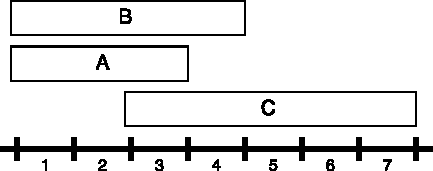
\includegraphics{abc.pdf}
\caption{Example with 7 time slots where peer A covers slots 1-3, peer B covers slots 1-4 and peer C covers slots 3-7}
\end{figure}

Because of this lack of symmetry, we no longer require peers to form reciprocal cliques. Instead, every peer finds its own replicas independently.\\

In the time-slot model, data availability of a single peer $p_1$ whose data is additionally replicated by peers $\{p_{2}, p_{3}, \ldots, p_{k}\}$ is equal to the sum of availabilities of $p_1, \ldots, p_k$, i.e. $A_1 \cup A_2 \cup \ldots \cup A_k$.\\
 
\section{Centralized approach}

% najpierw kliki - FPR

Let us begin with an optimization problem proposed by [KRZ] together with a proof of its NP-completeness.\\

An instance of the {\bf Fair Peer Replication} (FPR) problem consists of the set of peers $\{p_1,\ldots,p_n\}$ in a time-slot model with $T$ intervals. The optimization goal is to assign each peer to a clique, such that all the cliques are complete $(\forall G_k:A_{G_k} = \mathcal{T})$ and the size of the largest clique is minimized ($\min\max(|G_1|,\ldots,|G_N|)$).\\

The decision version of FPR is as follows. Given the set of peers' availabilities $\{A_i\}$, is it possible to assign each peer to exactly one clique such that all the cliques are complete and the size of the largest clique is at most $n$.

\begin{theorem}
FPR is NP-hard.
\end{theorem}
\begin{proof}

The proof is by reduction from GRAPH 3-COLORING. Given a graph $G$ we will first construct a larger graph $H$ that is 3-colorable if and only if $G$ is 3-colorable. Then we will construct an instance of FPR and a number $n$, such that the solution for this instance with largest clique of size at most $n$ exists if and only if $H$ is 3-colorable.\\

Given a graph $G$ with $k$ vertices and $m$ edges, we construct graph $H$ as follows. For each vertex $v_i\in V(G)$ there are three corresponding vertices $v^1_i, v^2_i, v^3_i \in V(H)$ connected by edges $(v^1_i, v^2_i); (v^2_i, v^3_i); (v^3_i, v^1_i) \in E(H)$ (we will refer to these as {\it joining} edges). For each edge $(v_p, v_q) \in E(G)$, there are three corresponding edges in $H$: $(v^1_p, v^1_q), (v^2_p, v^2_q), (v^3_p, v^3_q) \in E(H)$ (we will refer to them as {\it basic} edges). We also add $3k + 3m$ additional vertices $v^A_1,\ldots v^A_{3k+3m}\in V(H)$ that are not incident to any edges (we will refer to them as {\it free} vertices). The number of these additional free vertices $\{v^A_i\}$ is equal to the number of edges in $H$. We may bear in mind an implicit one-to-one correspondence between $\{v^A_i\}$ and $E(H)$ as it will be used in further constructions.\\

Graph $G$ is a subgraph of $H$ induced by the set of vertices $\{v^1_i\}$ so when a 3-coloring of $H$ is given, the 3-coloring of $G$ can be easily extracted. Conversely, when the 3-coloring of $G$ is given, it can be directly mapped into vertices from $\{v^1_i\}$. Colors of vertices from $\{v^2_i\}$ can be derived from $\{v^1_i\}$ by applying $(2,3,1)$ permutation to the color of each corresponding vertex. Similarly, colors for vertices from $\{v^3_i\}$ can be derived from $\{v^1_i\}$ by applying $(3,1,2)$ permutation to them. Vertices $\{v^A_i\}$ can be colored in any way because they are not incident to any edge. Thus, we get a coloring of graph $H$. Due to the permutations, in every triple $\{v^1_i, v^2_i, v^3_i\}$ there is exactly one vertex of each of the three colors. Moreover, permutations preserve the correctness of 3-coloring in subgraphs induced by $\{v^2_i\}$ and $\{v^3_i\}$, so the resulting 3-coloring of graph $H$ is correct.\\

Now we are going to construct an instance of FPR problem for graph $H$. Firstly, let us take $\mathcal{T} = \{1,\ldots,3k + 3m\}$, which is equal in size to $|E(H)|$. Each vertex of $H$ corresponds to a single peer $p_i$. We derive peers' availabilities based on pairs of interconnected vertices from $H$. The idea is that an edge corresponds to two peers that cannot belong to the same clique. For each peer $p_i$ we start with empty availability $A_i=\emptyset$. Then, for each edge $e_j = (v_p,v_q) \in E(H)$ (for $j = 1,2,\ldots,3k+3m$) we add $j$ to availability sets of peers corresponding to vertices $v_p$, $v_q$ and $v^A_j$. Vertex $v^A_j$ is the free vertex corresponding to edge $e_j$ as defined earlier. Observe that after the completion of the above method, each time slot is covered by exactly three peers.\\

To complete the proof, we will show that the answer to the FPR problem with peers' availabilities $\{A_i\}$ as defined above and $n=2k+m$ is positive if and only if graph $H$ is 3-colorable.\\

Let us firstly assume that the assignment to cliques with these constraints is possible. Notice that the number of peers (or $|V(H)|$) is equal to $3k+(3k+3m)=6k+3m=3n$. This means that the solution to FPR problem contains at least 3 cliques. On the other hand, each time slot is covered by exactly 3 peers so the number of cliques is at most 3, as all the cliques need to be complete. Thus, every solution to FPR consists of exactly 3 cliques and every time slot is covered by exactly one peer in each clique. Mapping clique IDs onto vertex colors leads to a 3-coloring of graph $H$. Suppose that the resulting 3-coloring is incorrect, i.e. there are two vertices $v_r$, $v_s$ of the same color connected by an edge $e_j$. This implies that peers $p_r$ and $p_s$ belong to the same clique. Time slot $j$ is covered by only three peers, two of which are in the same clique, which means that one of the other cliques does not cover time slot $j$, which leads to a contradiction.\\

Conversely, let us assume that $H$ is 3-colorable. When a 3-coloring of graph $H$ is given, it can be modified so that all colors are distributed equally among vertices. It is indeed the case in the subgraph induced by $\{v^1_i\} \cup \{v^2_i\} \cup \{v^3_i\}$ because in every triple $\{v^1_i, v^2_i, v^3_i\}$ there is exactly one vertex of each color. We can recolor the free vertices from $\{v^A_i\}$ in the following manner. For each edge $e_j=(v_p,v_q)\in E(H)$ we assign vertex $v^A_j$ the color that is assigned neither to $v_p$ nor to $v_q$. If $e_j$ is a basic edge, there exist three copies of it in $H$ with incident vertices of permuted colors. These three edges will commit three pairwise different colors to vertices from $\{v^A_i\}$. Similarly, if $e_j$ is a joining edge, it is one of three edges forming a $K_3$ subgraph out of vertices $\{v^1_i, v^2_i, v^3_i\}$. These three edges will also commit three pairwise different colors to vertices from $\{v^A_i\}$.
The resulting 3-coloring of $H$ can be directly mapped onto clique memberships. It will result in 3 cliques, each of size exactly $|V(H)| / 3 = n$. Moreover, every clique will be complete because due to recoloring every time slot is covered by exactly three peers of pairwise different colors. Thus, we have shown that the solution to our instance of the FPR problem exists.
\end{proof}

The FPR problem aims at achieving a state with perfect availability and minimizes the replication overhead. In real systems, perfect availability might be impossible to achieve within reasonable disk space limits. Moreover, we already argued that in the time-slot model, clique-based replication is not necessarily desirable. That is why we propose a different optimization problem.\\

An instance of the {\bf Uniform Peer Replication} (UPR) problem consists of the set of peers $\{p_1,\ldots,p_n\}$ in a time-slot model with $T$ intervals. Each peer has exactly $K$ replication slots available. The optimization goal is to assign exactly $K$ peers (replicas) to every peer so that each peer replicates exactly $K$ other peers and the sum of all resulting availabilities is maximized.\\

\textcolor{red}{TODO: podobny do 3-dimensinal assignment}

\section{De-centralized approach}

Results presented in the previous section suggest a conclusion that centralized optimization approaches to the replication problem can be computationally-heavy and also impractical for a few other reasons. Firstly, when a new peer joins the system or an existing peer decides to leave, the contracts need to be re-calculated. Secondly, if our goal is to maximize the overall state of the system, not considering differences between peers, highly-available peers have no incentives to be highly-available any more. They can rely on the system to provide them with appropriate replicators, which leads to a great loss of overall quality.\\

We would like to investigate a new, decentralized approach where peers communicate with one another and agree or disagree to replicate one another's data. Before that, let us briefly discuss an idea of a completely de-centralized game between peers proposed by \cite{krz} that works as follows. The set of players is equal to the set of peers and every player (peer) is selfish and thus interested only in maximizing availability of its own data. Game consists of an unlimited number of rounds. In each round, every peer enquires another peer of its choice to replicate its data (proposes a {\it replication contract}). In the subsequent rounds every peer answers to contract proposals (either accepts or rejects) and may also withdraw some of the existing contracts.\\

We decided that we would not aim at complete decentralization but allow a single central node to hold some valuable meta data. As we mentioned in section \ref{assumptions}, this central node will control truthfulness and openness of the system.\\

Since the time-slot model is not symmetric with respect to relative peers' contributions, we will not be relying on the idea of clique-based replication. Instead, every peer will do two distinct tasks: (a) ask other peers to replicate its data and (b) reply to replication requests from other peers with either acceptance or rejection. We do not require that if peer A replicates B's data, B has to replicate A's data. Thus, peers do not care whose data they replicate and their only concern is who is replicating their data. Peers are allowed to issue replication requests to any other peer at any point of time. To simplify, we assume that every peer has its own {\bf private measure} to rank other peers and uses the resulting order to select the best ones to enquire.\\

In terms of answering to requests, the logic of selecting peers that a given peer will replicate can be imposed by the system and uniform for every peer. There will be a system-wide {\bf acceptance measure} to rank requesting peers relatively to the peer that is answering. It is worth noting that control over peers following that imposed logic is fairly easy to implement as all the replication contracts may be public and registered in the central node. The central node will verify if the peers are following the imposed measure to accept requests and punish the cheaters.\\


Let us formalize the notion of measure that we informally introduced and also emphasise the distinction between the two above-mentioned measures.

\begin{definition}
A {\bf peer measure} (or just measure) is a function from a pair of peers (replica and requester) to an integer. The integer value denotes how good it is for a replica to replicate requester's data.
\end{definition}

We will later be interested in measures that are fair.

\begin{definition}
A measure is {\bf fair} if lowering requesters availability cannot increase the measure value.
\end{definition}

Using measures that are not fair will lead to lack of incentives and overall system instability. We distinguish between two types of measures, used in two different situations.\\

\begin{definition}
The {\bf acceptance} measure (AM) is the peer measure used by a peer to rank other peers asking for data replication and select exactly K of them, where K is the number of replication slots. The acceptance measure is imposed by the system and peers are obliged to use it.\\
\end{definition}

\begin{definition}
The {\bf private} measures (PM) are all the peer measures used by peers to select potential replicators of their data and issue a replication request to them. Only if a replicator decides that the querying peer is among K best peers according to acceptance measure, the data will be replicated. Every peer can use any seeker measure it prefers.\\
\end{definition}

Private measures are secret to peers so they can be chosen arbitrarily and even changed over time to adapt to changing system conditions. However, realistically, peers will be always selfishly interested in maximizing availability of their data. Since we do not have any control over the measures, we make a simplifying assumption that every peer chooses replicators to query in a way that will maximize their availability {\bf in their current situation}. Precisely - every peer in any moment of time will ask the single replica that (if successful) will lead to highest time-slot coverage (possibly after removing some other currently co-operating replica if all replication slots are taken).\\

We are interested in analysing only the acceptance measure, which is the key factor of system's performance. Manipulating the acceptance measure is a way to shift the equilibrium in favour of either better or worse peers. Let us analyse two simple examples that represent two extremes.\\

% chyba nie jest jasne jaki to "stronger" peer - zdefiniuj strength przy definicjach modeli

{\bf Example \#1}\\
Let us assume for a moment that the acceptance measure is chosen to be equal to the sum of time-slots covered by the requester.
$$AM_{strong}(p_i) = |A_i|$$
This way clearly favours stronger peers as they will be always accepted by the replicators if competing with weaker ones. Also $AM_{strong}$ is clearly a fair measure.\\

{\bf Example \#2}\\
On the other hand, let us think of a system measure being equal to the amount of slots that a replicator will add to what the requester is already covering.
$$AM_{weak}(p_i) = |A_r \cap A_i|$$
where $A_r$ means replicator's availability.
Such solution will favour weaker peers. Thus, highly-available peers lose incentives to be highly-available and might try to lower their advertised availability in order to get better replicas from the system.\\

We can see that both of these measures lead to some imbalance in the system. That is why we will try using hybrids of the above-mentioned measures.\\

{\bf Example \#3}\\
The most natural of such hybrids is a simple sum of the measures from examples 1 and 2.
$$AM_{sum}(p_i) = |A_i| + |A_r \cap A_i|$$
This measure does not have the disadvantage from example 2. Peers have no incentives to lower their availability because their gain can be at most zero ($AM_{sum}$ is fair). Also the whole system is not biased towards the best peers.\\

\textcolor{red}{TODO: tutaj wstawie rysunek podobny do tego, ktory narysowalem na tablicy i powiem o liniowych kombinacjach dwoch powyzszych skladnikow w mierze. Musze tez jeszcze rozwazyc nieliniowe kombinacje.}\\

% Przyklad, ze miary zalezne od sytuacji prowadza do cyklu

%
%
%  ----------- CHAPTER 4 -----------------------------------------------
%
%

\chapter{Experiments}\label{chap:experiments}

Last chapter of this work is devoted to analysing outcomes of the simulations and real-life deployments of Nebulostore with various replicating strategies that we discussed in chapter 3.
Before conducting any experiments, we need to know what are the expected peers' capabilities in terms of disk space and availability. When it comes to disk space, authors of \cite{farsite} suggest that disk capacities are increasing faster than storage needs. Since in early 2000s estimated percentage of unused disk space on an average corporate workstation was above 50\%, we can safely assume that space requirements for data replication are easily fulfilled. \textcolor{red}{TODO czy jest sens pisac o early 2000s?}
On the other hand, peer availability is a more complex issue, which we need to research more thoroughly before formulating any assumptions. \\

\section{Peer behaviour in real systems}

We begin with reviewing existing results of availability analyses based on trace data from real P2P systems that gained popularity. We focus on three distinct cases in which peer behaviour is dissimilar due to the nature of the systems and their participants. We distinguish between file-sharing services, such as Napster, volunteer-computing efforts based on BOINC platform, such as SETI@HOME, and a backup system deployed in a university computer lab.\\

\subsection{P2P file-sharing services analysis}

There are a few analyses of traces from P2P file-sharing systems, which popularity peaked in early 2000s, namely Napster, eDonkey and Gnutella. The authors of \cite{napster} used crawlers to study Napster and Gnutella networks over a period of a few consecutive days (4 and 8 respectively). The results regarding availability for both systems were similar. Average peer availability was less than 20\%. Half of the peers never remained on-line for more than one hour and 26\% of users never shared any data. This behaviour is typical to {\it free-riders} --- peers that use the system but do not contribute any resources. The only significant difference between Gnutella and Napster was among the best clients. Best 20\% of Napster hosts had uptime of 83\% or more while best 20\% of Gnutella hosts had uptime of only 45\% or more.\\

The authors of \cite{edonkey} claim to have traced 14 million eDonkey peers over the period of 27 days. They came to a similar conclusion that peers who were in the system for at least 10 days had 20\% availability on average. They also discovered that peer sessions were long, 9 hours on average, but with high variance. Over half of the peers had the average session length of 3 hours or less.\\

We can observe that a significant number of peers tend to connect only to download files (probably also uploading some content during this period) and disconnects immediately after they have obtained them. We do not think this will be a typical behaviour of NebuloStore clients.\\

\subsection{BOINC systems analysis}

BOINC (Berkeley Open Infrastructure for Network Computing) is a freely-available middleware for deploying volunteer computing projects, such as SETI@HOME. It made its traces publicly available allowing interesting analyses to be performed by researchers. Papers \cite{availability} and \cite{seti} analyse data from 1.5 years of SETI@HOME activity (years 2007-2008), which consists of 57 thousand years of CPU time, 102 million of availability intervals and over 330 thousand hosts.\\

The most interesting contribution of \cite{availability} is an attempt to classify peers into clusters of similar patterns of availability. Authors came to a conclusion that 90\% of peers are always on or always off and the remaining 10\% of peers can be further divided into groups that represent either cyclic behaviour (correlated with hours in a day or days in a week) or behave randomly. Consistently, authors of \cite{seti} claim that about 6\% of peers have deterministic, cyclic patterns of availability. Furthermore, longest 20\% of availability intervals contribute to 90\% of overall availability, which means that the core of BOINC is made of highly-available peers.\\

Another independent analysis \cite{storage} points out that the average availability of SETI@HOME machines is 81\%. The average host lifetime before experiencing a permanent failure is 91 days. When it comes to disk space, it is normally distributed with an average of 50\% of disk space available.\\

It is worth noting that BOINC has in fact a client-server architecture, not a P2P one. However, we still consider the behaviour of BOINC clients to be closely related to NebuloStore clients' behaviour.\\

\subsection{Backup system deployment}

Another interesting deployment is presented in \cite{hetero}. A backup system similar to Nebulostore was installed in a university computer lab and also in the PlanetLab environment. Authors claim that the main factor contributing to system's quality and efficiency is the availability of hosts. In the university lab deployment, the average availability of the machines was only 13\% and transient failures were very frequent. However, with the help of asynchronous messaging, auhors were able to a`chieve overall stability. Average times of creating the first, the second and the third replica of a file ware equal to, respectively, 1.1h, 2.7h and 5.5h.\\

\textcolor{red}{czy jeszcze jakies wnioski? Czy napisac ze ten projekt byl w jakis sposob zwiazany z Nebulo, byl jego bratem lub przodkiem?}

\section{Simulations}

\textcolor{red}{symulujac warunki wynikajace z powyzszych prac}

 
 
%Other notes and ideas
%http://en.wikipedia.org/wiki/CAP_theorem

\chapter{Summary and Conclusions}\label{chap:conclusions}


%
%
%  ----------- BIBLIOGRAPHY -----------------------------------------------
%
%


\bibliographystyle{plainnat}
\bibliography{mgr}

\end{document}
